% This is a template I made based on my (successful) Goldwater Scholarship application research essay. The formatting should be correct as of the 2019 application cycle, so check to make sure it lines up with any possible changes made since then. At the time, these were their formatting guidelines:
% - 12 pt Arial font
% - 1 inch margins on all sides (but headers and page numbers can encroach within the margins)
% - no longer than 3 pages total
% - your name and university at the top of each page
% - captions for figures may be in 10 pt Arial font

% I am not responsible for any repercussions you have from using this template. Use it at your own risk. My advice is based on my own reasoning, so take it as you will.

% Hannah W. Richards
% hannah_banana98@protonmail.com
% thrichards@crimson.ua.edu
% June 3, 2019
% Revised August 28, 2020

% I don't care what the output of using this template looks like, i.e. you don't have to attribute me or mention anything about the template in the generated PDF that you submit to Goldwater. If you modify this template and release it as a separate .tex file, however, please attribute me in the header.

% All the text and figures of this template were created by me and my own.

% Now, onto some tips and tricks I have.
% I trust that you've read the official application tips and guidelines for the Goldwater research essay. If you haven't, they're pretty easy to find on the website.
% The research essay is a bit of an odd paper to write. It is, at some level, a scientific paper, much like a journal article. However, it is simultaneously something of a personal statement, as its goal is to sell YOU, not your research.
% Generally, I suggest you use first-person singular pronouns throughout your essay, especially in the "methods" section. This deviates from the norm in academic journals, where you'll generally use plural first-person pronouns, even if it was you alone who did the work. The idea here is that you can clearly describe the work that YOU did, and there won't be a question of how much of a role you had in a collaboration.
% Your readers will have general scientific knowledge, but you can't expect them to know specific details about your field. This means that they will *most likely* be familiar with terms and concepts found in introductory college courses. For example, you probably don't need to define words and phrases like isotope, carbohydrate, standard deviation, resistor, beta decay, etc. You'll probably want to explain what a Grand Unified Theory is, however.
% The essay may seem daunting at first, but pretty soon you're going to wish you had more space. Three pages fill up surprisingly quickly. You'll probably have your best results borrowing from a paper or report you've already written and condensing it down to its bare components. Play around with the formatting a bit until you have everything on three pages.
% I used two columns, which is what my campus representative recommended. It's easier to read, and figures take up less space, which means you can have a more compact paper.

\documentclass[12pt, letterpaper, twocolumn]{article}
\usepackage[margin=1.0in]{geometry}
\usepackage{fontspec}
\setmainfont{Arial}
\usepackage{fancyhdr}
\setlength{\headheight}{14.5pt}
\usepackage{graphicx}
\usepackage{caption}
\captionsetup[figure]{font=small}
\usepackage{amsmath}
\usepackage[]{siunitx}
\usepackage[style=numeric,sorting=none]{biblatex}
\addbibresource{references.bib}
\pagestyle{fancy}
\fancyhf{}
\lhead{Your Name} % change this to your actual name
\rhead{Your University} % same for your university
\rfoot{\thepage}

\begin{document}

% title
\begin{center}
\textbf{A Complete Yet Concise Title For Your Research Project}
\end{center}

% introduction
\noindent\textbf{Introduction}\\
Background information necessary for the reader to understand the content of the rest of the paper. Your reader will be familiar with general scientific terms, but jargon should be defined here or avoided (if reasonably achievable). See Table~\ref{table:ExampleTable} for an example table.

% tables, if needed, are like this.
\begin{table}[ht]
\begin{tabular}{|l|l|l|}
\hline
Time (s) & Distance (m) & Charge (C) \\ \hline
0        & 0            & 10         \\ \hline
1        & 1            & 5          \\ \hline
2        & 4            & 6          \\ \hline
\end{tabular}
\caption{An example table.}
\label{table:ExampleTable}
\end{table}

\vspace{0.125in}
% methods
\noindent\textbf{Methods}\\
Describe the specific steps you took to obtain the results you did. Maybe include a figure or blocks of (pseudo) code. See Figure~\ref{fig:ExampleFigure}.
% figure: you'll probably have multiple figures. i had 5. you can use this basic formatting scheme for each one.
% it usually doesn't hurt to use a vectorized image format like .pdf or (if you can get it to work here) .svg. otherwise, .png is fine. it's what i used for pretty much all my figures.
\begin{figure}[ht]
    \centering
    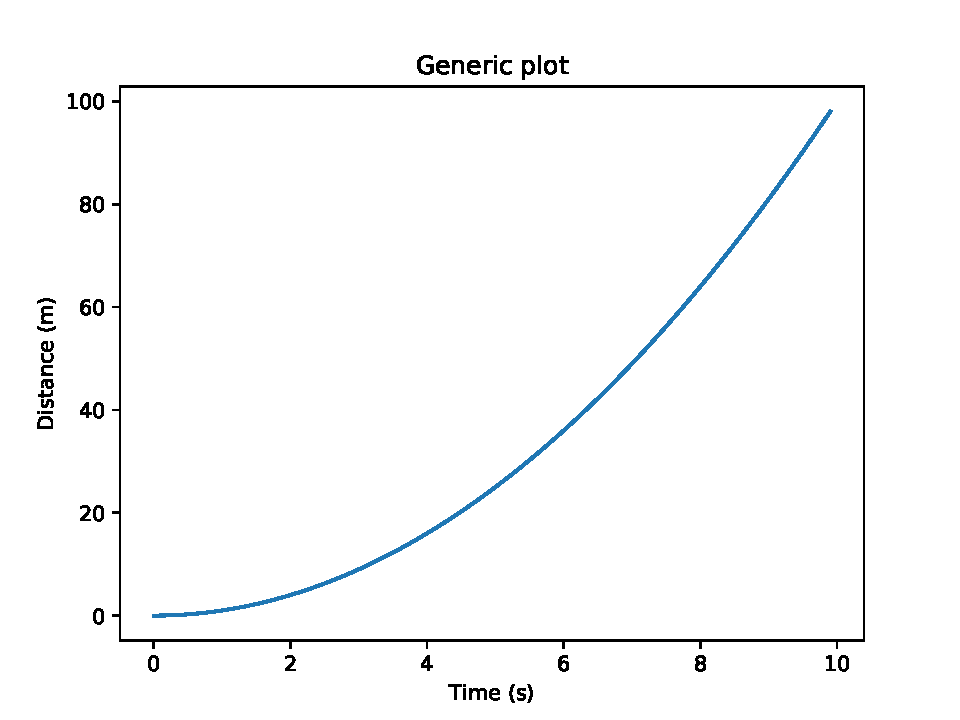
\includegraphics[width=0.5\textwidth]{img/generic_plot.pdf}
    \caption{Here is a caption for a figure.}
    \label{fig:ExampleFigure}
\end{figure}
Footnotes always look nice.~\footnote{This is a footnote.}

Try to keep equations to a minimum. Sorry, theorists. FYI, math isn't going to show up in Arial font, which should still be okay. See Equation~\ref{eqn:ExampleEquation}.
\begin{equation}
    \sum_{i=0}^n c_i x_i = c_0 x_0 + c_1 x_1 + ... + c_n x_n
\label{eqn:ExampleEquation}
\end{equation}

The methods section is the place to show off the skills you learned while working on the project and demonstrate scientific reasoning. A good way of doing this is to explain confounding factors in your research and how you overcame them. This will probably be your longest section.

\vspace{0.125in}
% results
\noindent\textbf{Results}\\
Discuss your final findings here. The bulk of this section will likely be multiple figures. See Figure~\ref{fig:AnotherFigure}, and remember to reference all the figures and tables you have in your essay.

\begin{figure}[ht]
    \centering
    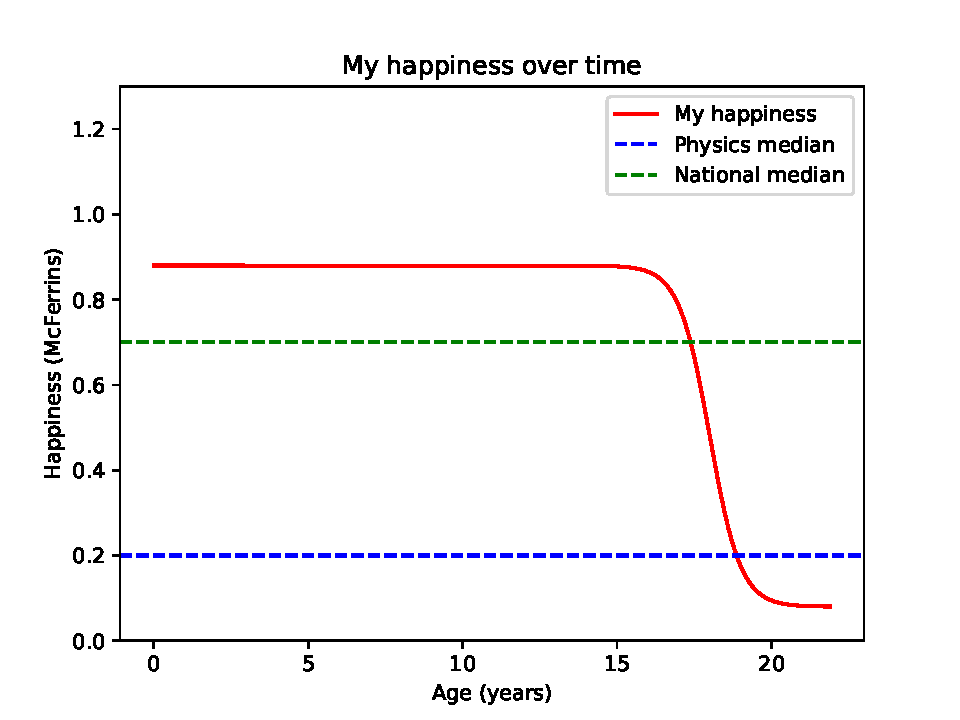
\includegraphics[width=0.5\textwidth]{img/happiness_plot.pdf}
    \caption{haha. (I'm doing a lot better now, don't you worry.)}
    \label{fig:AnotherFigure}
\end{figure}

Remember to cite your sources throughout the paper~\cite{this_article}.

\vspace{0.125in}
% conclusion
\noindent\textbf{Conclusion}\\
Respond to your introduction and discuss the implications of your results. Maybe a preliminary plot of some future expected findings.

\vspace{0.125in}
% future studies
\noindent\textbf{Future Studies}\\
Here you'll have the next steps you'll take in your research. If your next project is not a continuation of this project, try to find a way to link them together. A good way is to discuss the skills you gained from this project and how you'll apply them in the future (especially still as an undergrad). If you're diverting quite a bit from this project, use some key words like ``broaden.'' If you're continuing in the same field, ``deepen.''

\vspace{0.125in}
%\newpage
% references: this should be automatic. you can also cut out extra info (titles, websites) if you're running out of space. i used 7 references in my essay, so take that info as you will.
\noindent\textbf{References}
\vspace{-0.125in}
\printbibliography[heading=none]

\end{document}
